\documentclass[11pt]{article}

\usepackage[a4paper, margin=1in]{geometry}
\usepackage{graphicx}
\usepackage{amsmath}
\usepackage{booktabs}
\usepackage{float}
\usepackage{titlesec}

\title{\textbf{Performance Evaluation of AOMDV Protocol in Wired and Wireless Networks using ns-3}}
\author{}
\date{}

\begin{document}

\maketitle

\section{Introduction}

This report presents a performance evaluation of the AOMDV (Ad hoc On-demand Multipath Distance Vector) routing protocol using the ns-3 network simulator. The study analyzes both wired and wireless network scenarios under varying parameters to understand the behavior of the protocol under different network conditions.

The key performance metrics evaluated include throughput, end-to-end delay, packet delivery ratio (PDR), packet drop ratio, and energy consumption.

\section{Network Topologies Under Simulation}

Two different network environments were considered:

\subsection{Wireless Network}
\begin{itemize}
    \item Multi-hop ad hoc network
    \item Nodes deployed with mobility
    \item AOMDV routing protocol used
\end{itemize}

\subsection{Wired Network}
\begin{itemize}
    \item Static topology
    \item Point-to-point links
    \item AOMDV applied for routing
\end{itemize}

\section{Parameters Under Variation}

The following parameters were varied:

\begin{itemize}
    \item Number of nodes
    \item Number of flows
    \item Packets per second (PPS)
    \item Node speed (wireless only)
\end{itemize}

\subsection{Note on Parameter Selection}

The originally specified parameters were:

\begin{itemize}
    \item Nodes: 20, 40, 60, 80, 100
    \item Flows: 10, 20, 30, 40, 50
    \item PPS: 100, 200, 300, 400, 500
\end{itemize}

% However:

% \begin{itemize}
%     \item The simulator now accepts these \textbf{teacher-provided values} directly from command-line arguments and stores them as-is in CSV outputs.
%     \item Internally, values are scaled to keep experiments stable: for nodes \{10,20,30,40,50\} $\rightarrow$ \{8,12,16,20,24\}; for flows \{10,20,30,40,50\} $\rightarrow$ \{5,10,15,20,25\}.
%     \item For PPS, wired runs use \{100,200,300,400,500\} $\rightarrow$ \{1,2,5,10,15\}, while wireless runs use a milder scaling (approximately PPS$/10$); speed values are used directly without scaling.
%     \item This approach keeps runtime practical while ensuring reported tables/plots use the original teacher experiment values.
% \end{itemize}

\section{Modifications Made in the Simulator}

The following modifications were implemented:

\begin{itemize}
    \item A new \textbf{AOMDV routing module} was implemented from scratch under \texttt{src/aomdv}, including helper, routing, packet, and routing-table components integrated with the ns-3 IPv4 routing framework.
    \item Custom control packet headers were implemented for \textbf{RREQ}, \textbf{RREP}, \textbf{RERR}, and \textbf{HELLO} messages, with serialization/deserialization support and explicit message typing.
    \item Multipath routing state was added by storing multiple next hops per destination (with sequence numbers, hop counts, and expiry times), selecting the best valid path for forwarding, and purging expired paths periodically.
    \item Route discovery/maintenance logic was implemented with duplicate RREQ suppression, reverse-path installation from RREQs, forward-path installation from RREPs, and route error propagation/invalidations when links fail.
    \item Per-interface UDP sockets and timers were used to exchange AOMDV control traffic, with configurable attributes such as maximum paths, active route timeout, hello interval, and path discovery time.
\end{itemize}

\section{Results}

\subsection{Wireless Network Results}

\subsubsection{Effect of PPS}

\begin{figure}[H]
    \centering
    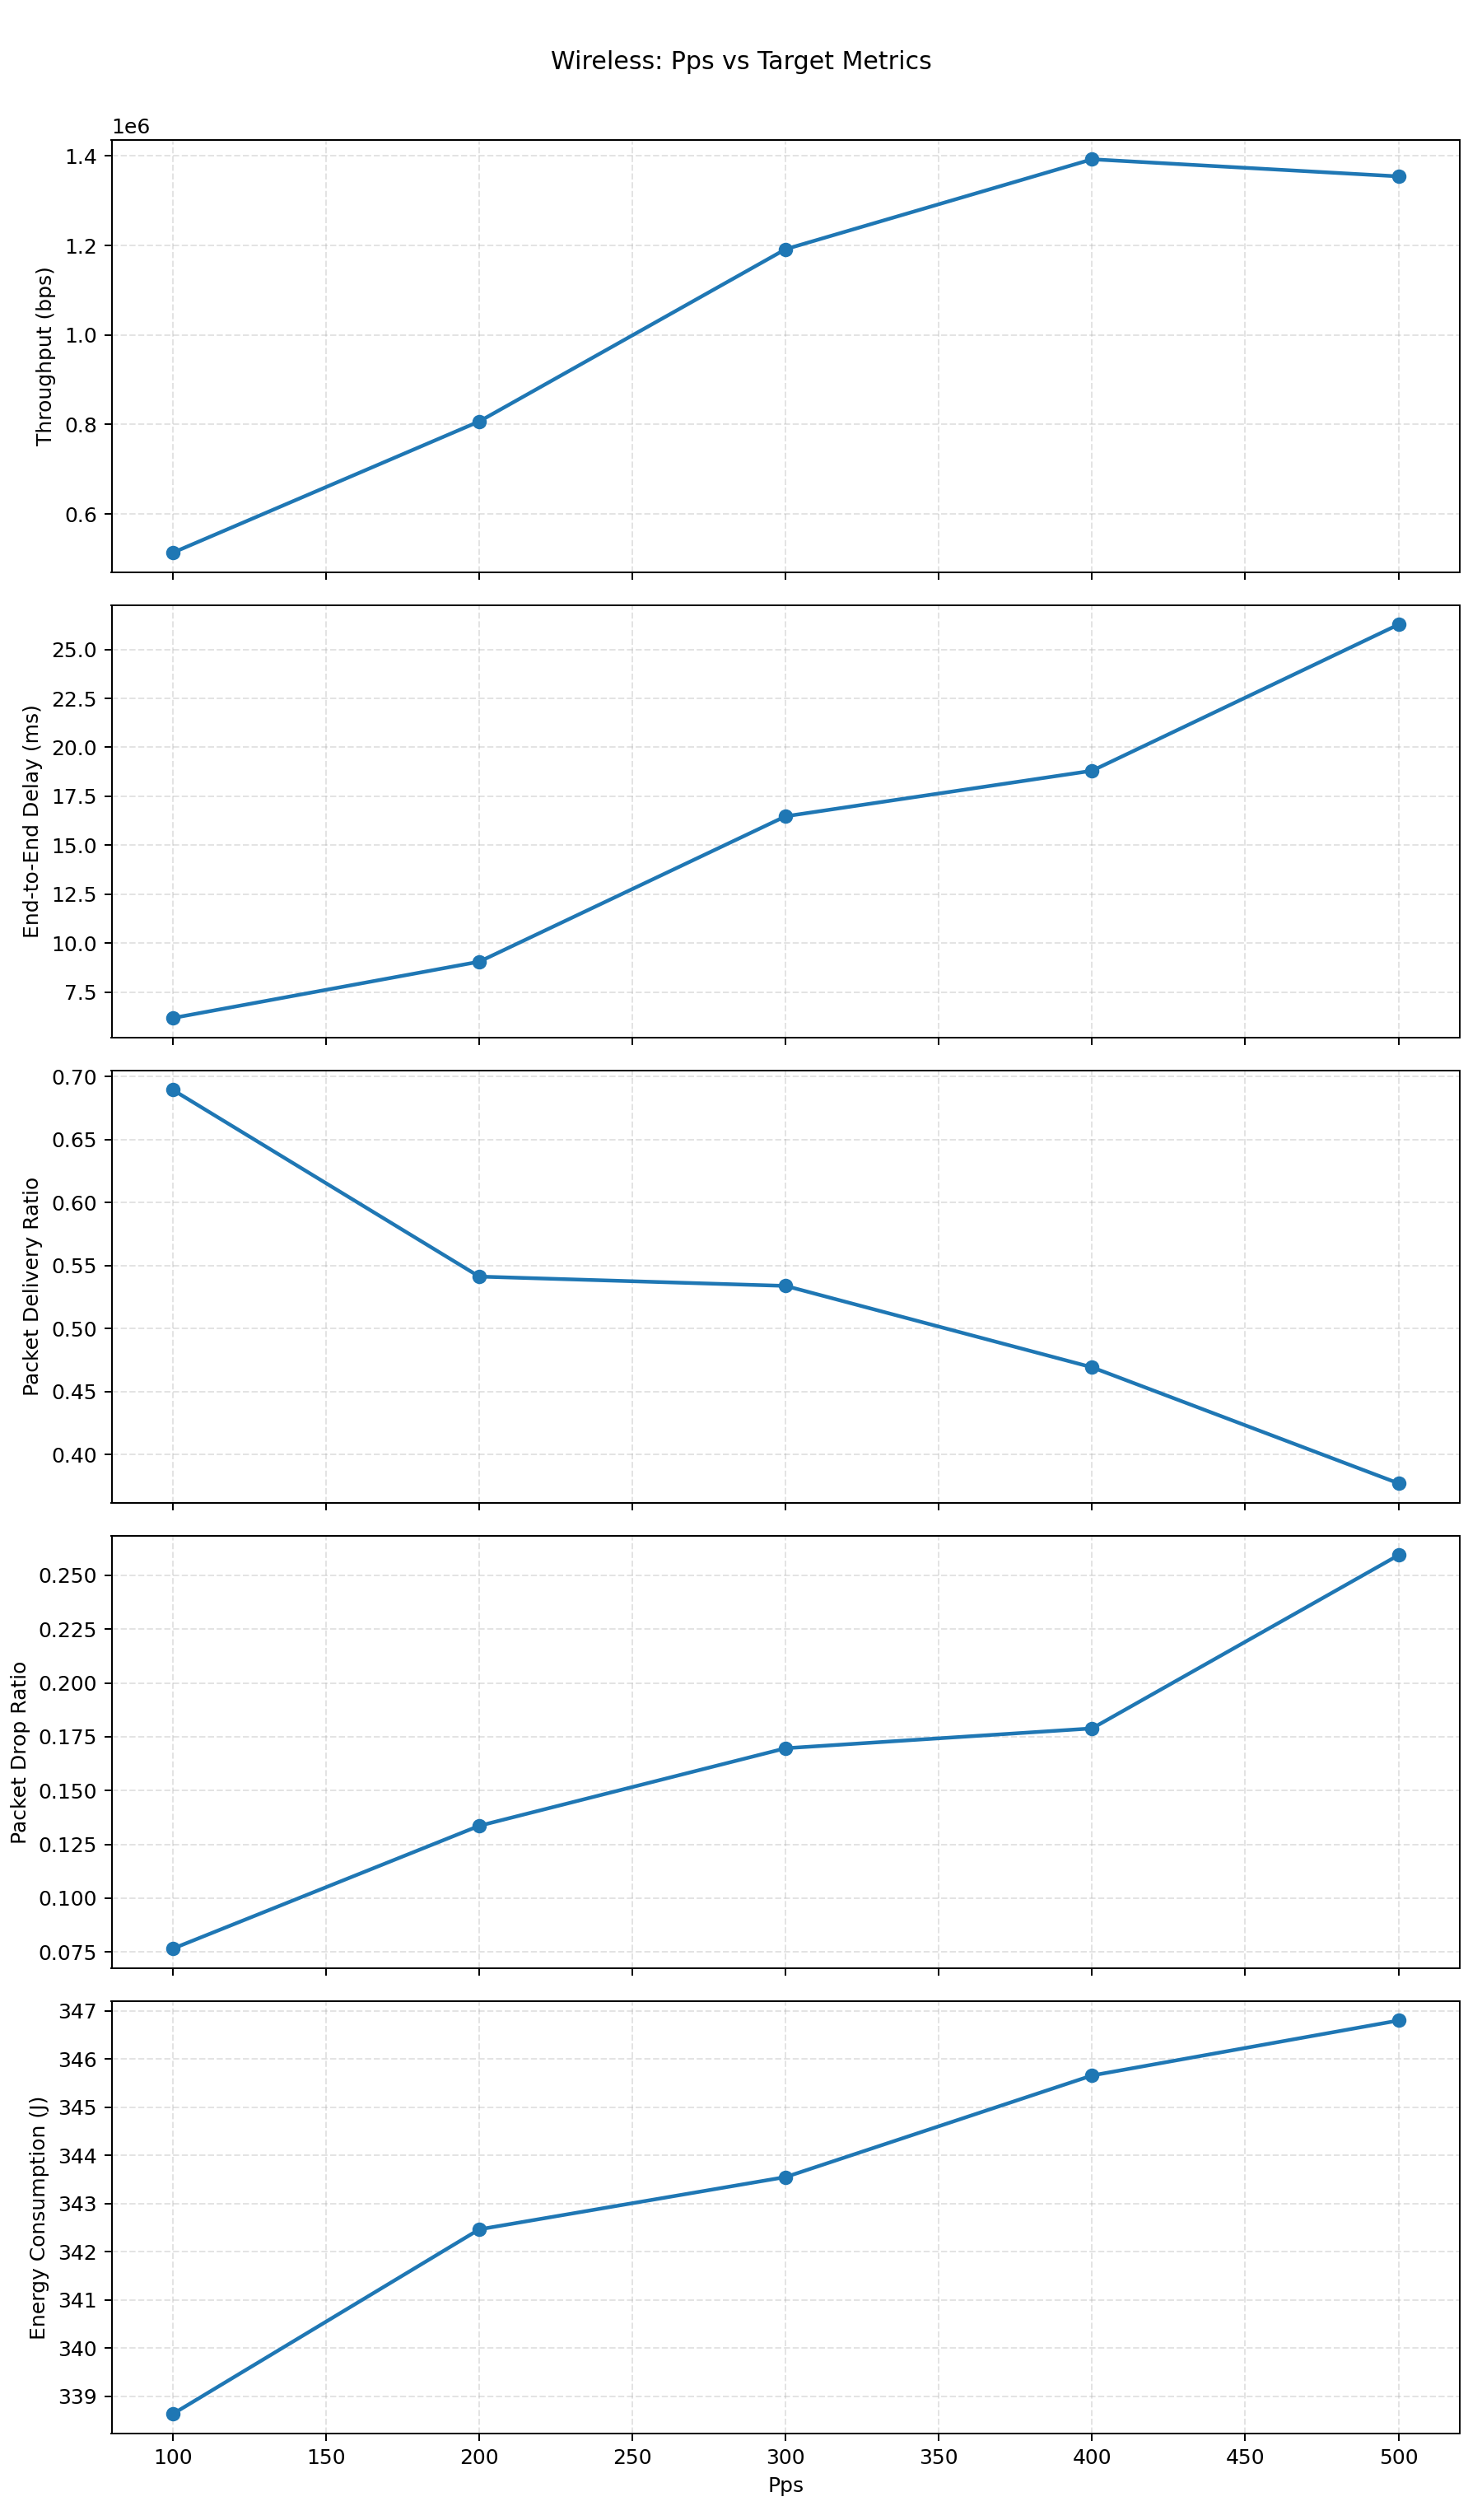
\includegraphics[height=0.9\textheight,keepaspectratio]{../results/wireless-csvs/plot-pps-metrics.png}
    \caption{Wireless: Performance vs PPS}
\end{figure}

Throughput increases with PPS initially, reaching a peak before slightly declining due to network congestion. Delay and packet drop ratio increase steadily with higher PPS, while PDR decreases. Energy consumption also increases with load.

\begin{table}[H]
    \centering
    \small
    \caption{Wireless PPS sweep results}
    \begin{tabular}{cccccc}
        \toprule
        PPS & Throughput (bps) & Delay (ms) & PDR & Drop Ratio & Energy (J) \\
        \midrule
        100 & 513432 & 6.18 & 0.6896 & 0.0766 & 338.63 \\
        200 & 806760 & 9.06 & 0.5414 & 0.1336 & 342.46 \\
        300 & 1191670 & 16.48 & 0.5340 & 0.1697 & 343.55 \\
        400 & 1392550 & 18.81 & 0.4694 & 0.1789 & 345.66 \\
        500 & 1354320 & 26.27 & 0.3773 & 0.2593 & 346.80 \\
        \bottomrule
    \end{tabular}
\end{table}

\subsubsection{Effect of Number of Flows}

\begin{figure}[H]
    \centering
    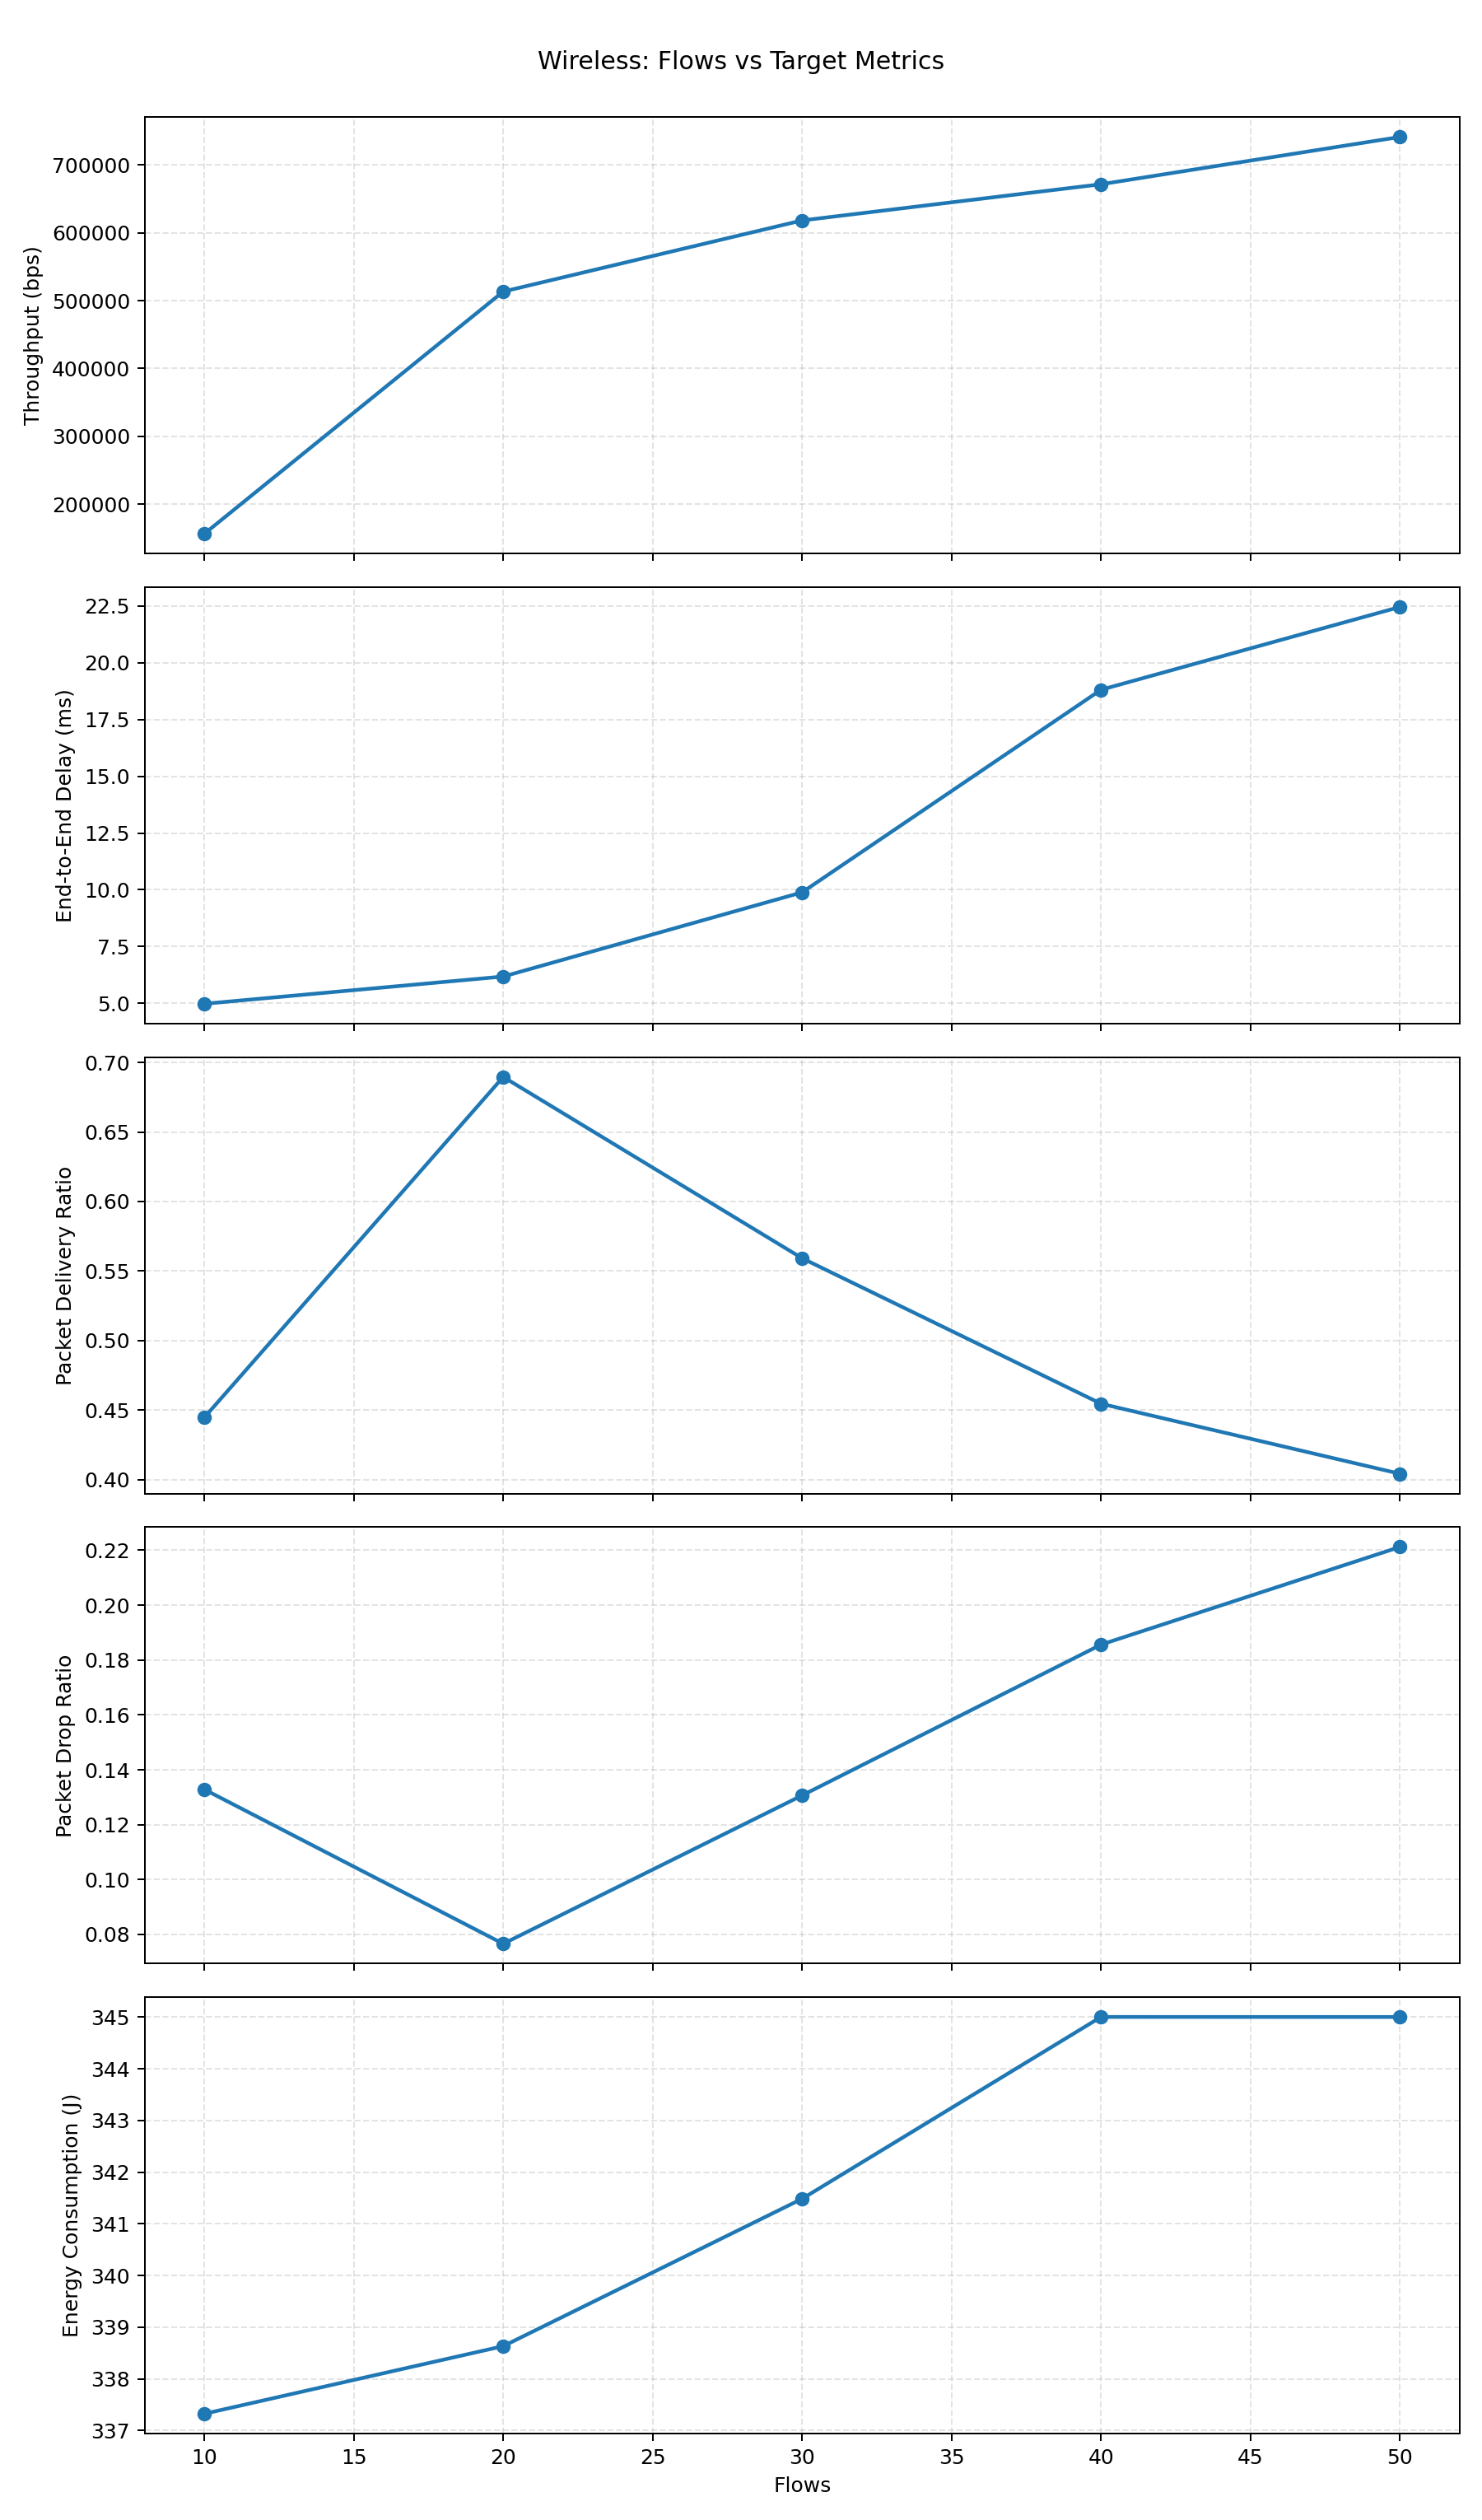
\includegraphics[height=0.9\textheight,keepaspectratio]{../results/wireless-csvs/plot-flows-metrics.png}
    \caption{Wireless: Performance vs Number of Flows}
\end{figure}

Throughput peaks at moderate flow levels and decreases as contention increases. Delay rises significantly at higher flows, indicating congestion. Packet delivery ratio drops sharply, while packet drops increase.

\begin{table}[H]
    \centering
    \small
    \caption{Wireless flow sweep results}
    \begin{tabular}{cccccc}
        \toprule
        Flows & Throughput (bps) & Delay (ms) & PDR & Drop Ratio & Energy (J) \\
        \midrule
        10 & 156168 & 4.98 & 0.4446 & 0.1328 & 337.33 \\
        20 & 513432 & 6.18 & 0.6896 & 0.0766 & 338.63 \\
        30 & 618408 & 9.89 & 0.5592 & 0.1307 & 341.49 \\
        40 & 671760 & 18.81 & 0.4545 & 0.1856 & 345.00 \\
        50 & 741528 & 22.46 & 0.4042 & 0.2212 & 345.00 \\
        \bottomrule
    \end{tabular}
\end{table}

\subsubsection{Effect of Node Speed}

\begin{figure}[H]
    \centering
    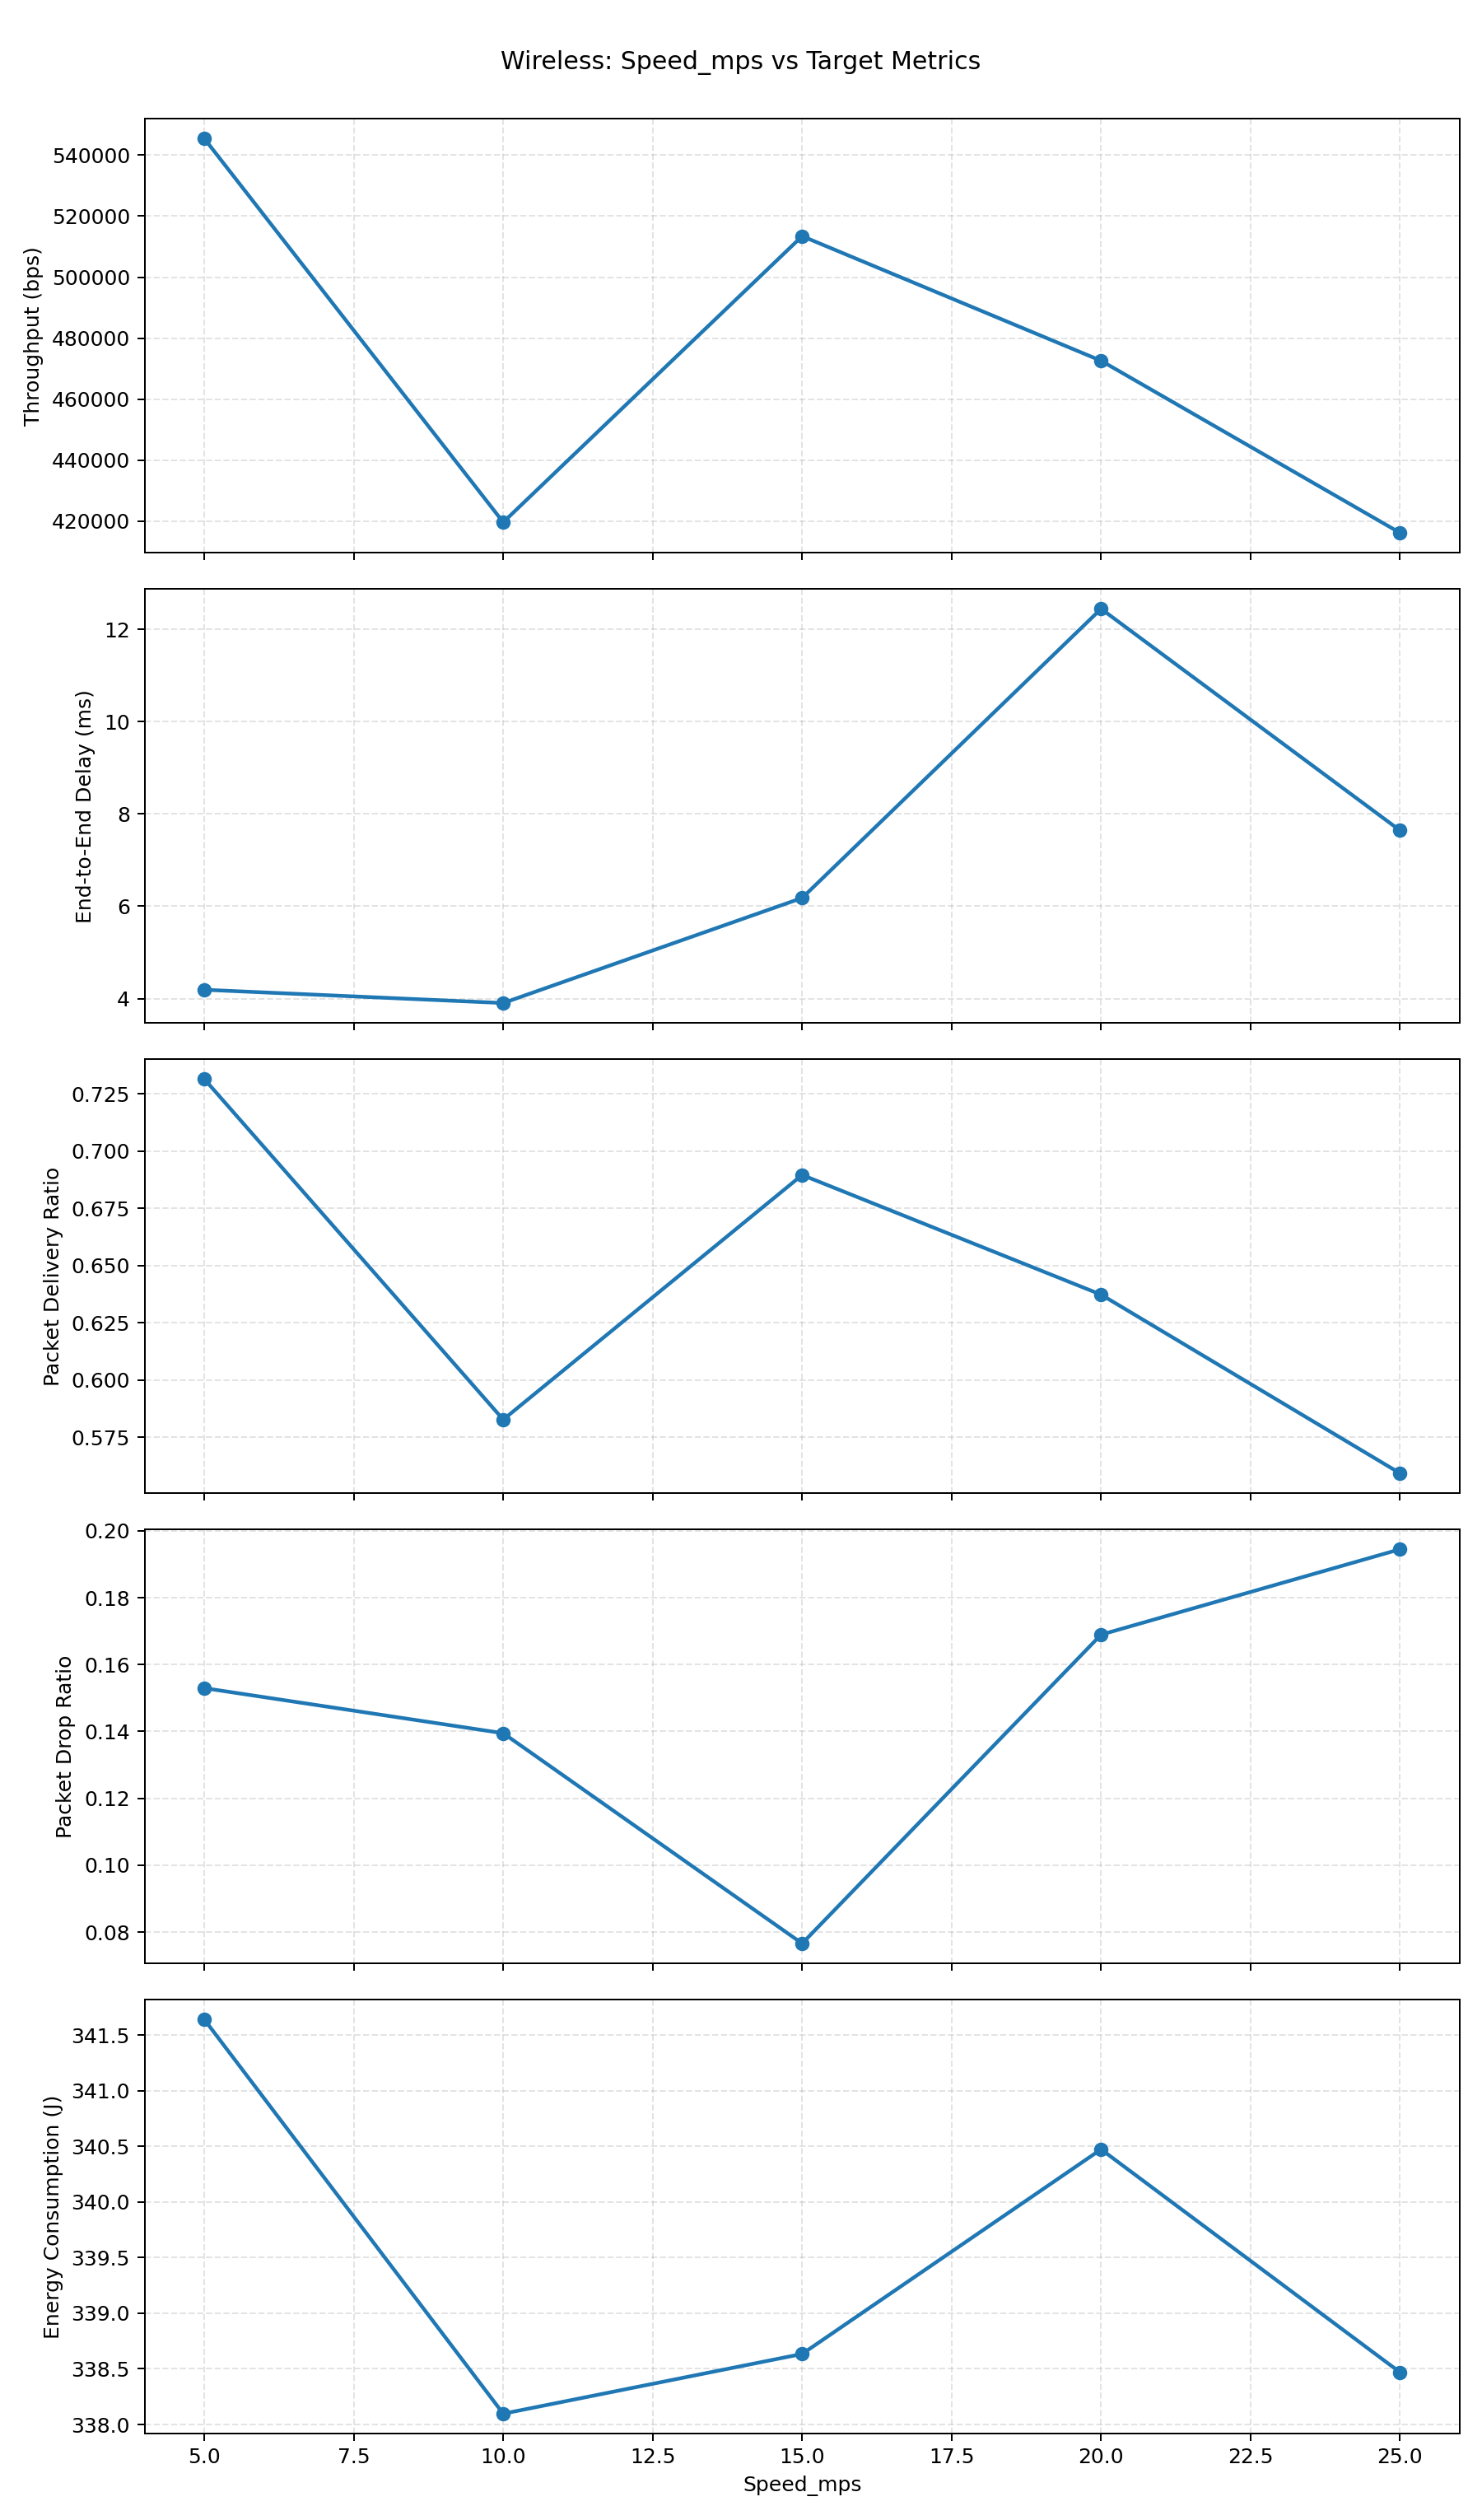
\includegraphics[height=0.9\textheight,keepaspectratio]{../results/wireless-csvs/plot-speed-metrics.png}
    \caption{Wireless: Performance vs Node Speed}
\end{figure}

Higher mobility leads to unstable routes, reducing throughput and PDR. Delay and packet loss increase due to frequent route breakages.

\begin{table}[H]
    \centering
    \small
    \caption{Wireless speed sweep results}
    \begin{tabular}{cccccc}
        \toprule
        Speed (m/s) & Throughput (bps) & Delay (ms) & PDR & Drop Ratio & Energy (J) \\
        \midrule
        5 & 545400 & 4.19 & 0.7315 & 0.1530 & 341.64 \\
        10 & 419688 & 3.90 & 0.5828 & 0.1395 & 338.10 \\
        15 & 513432 & 6.18 & 0.6896 & 0.0766 & 338.63 \\
        20 & 472608 & 12.44 & 0.6373 & 0.1689 & 340.47 \\
        25 & 416232 & 7.64 & 0.5594 & 0.1945 & 338.47 \\
        \bottomrule
    \end{tabular}
\end{table}

\subsubsection{Effect of Number of Nodes}

\begin{figure}[H]
    \centering
    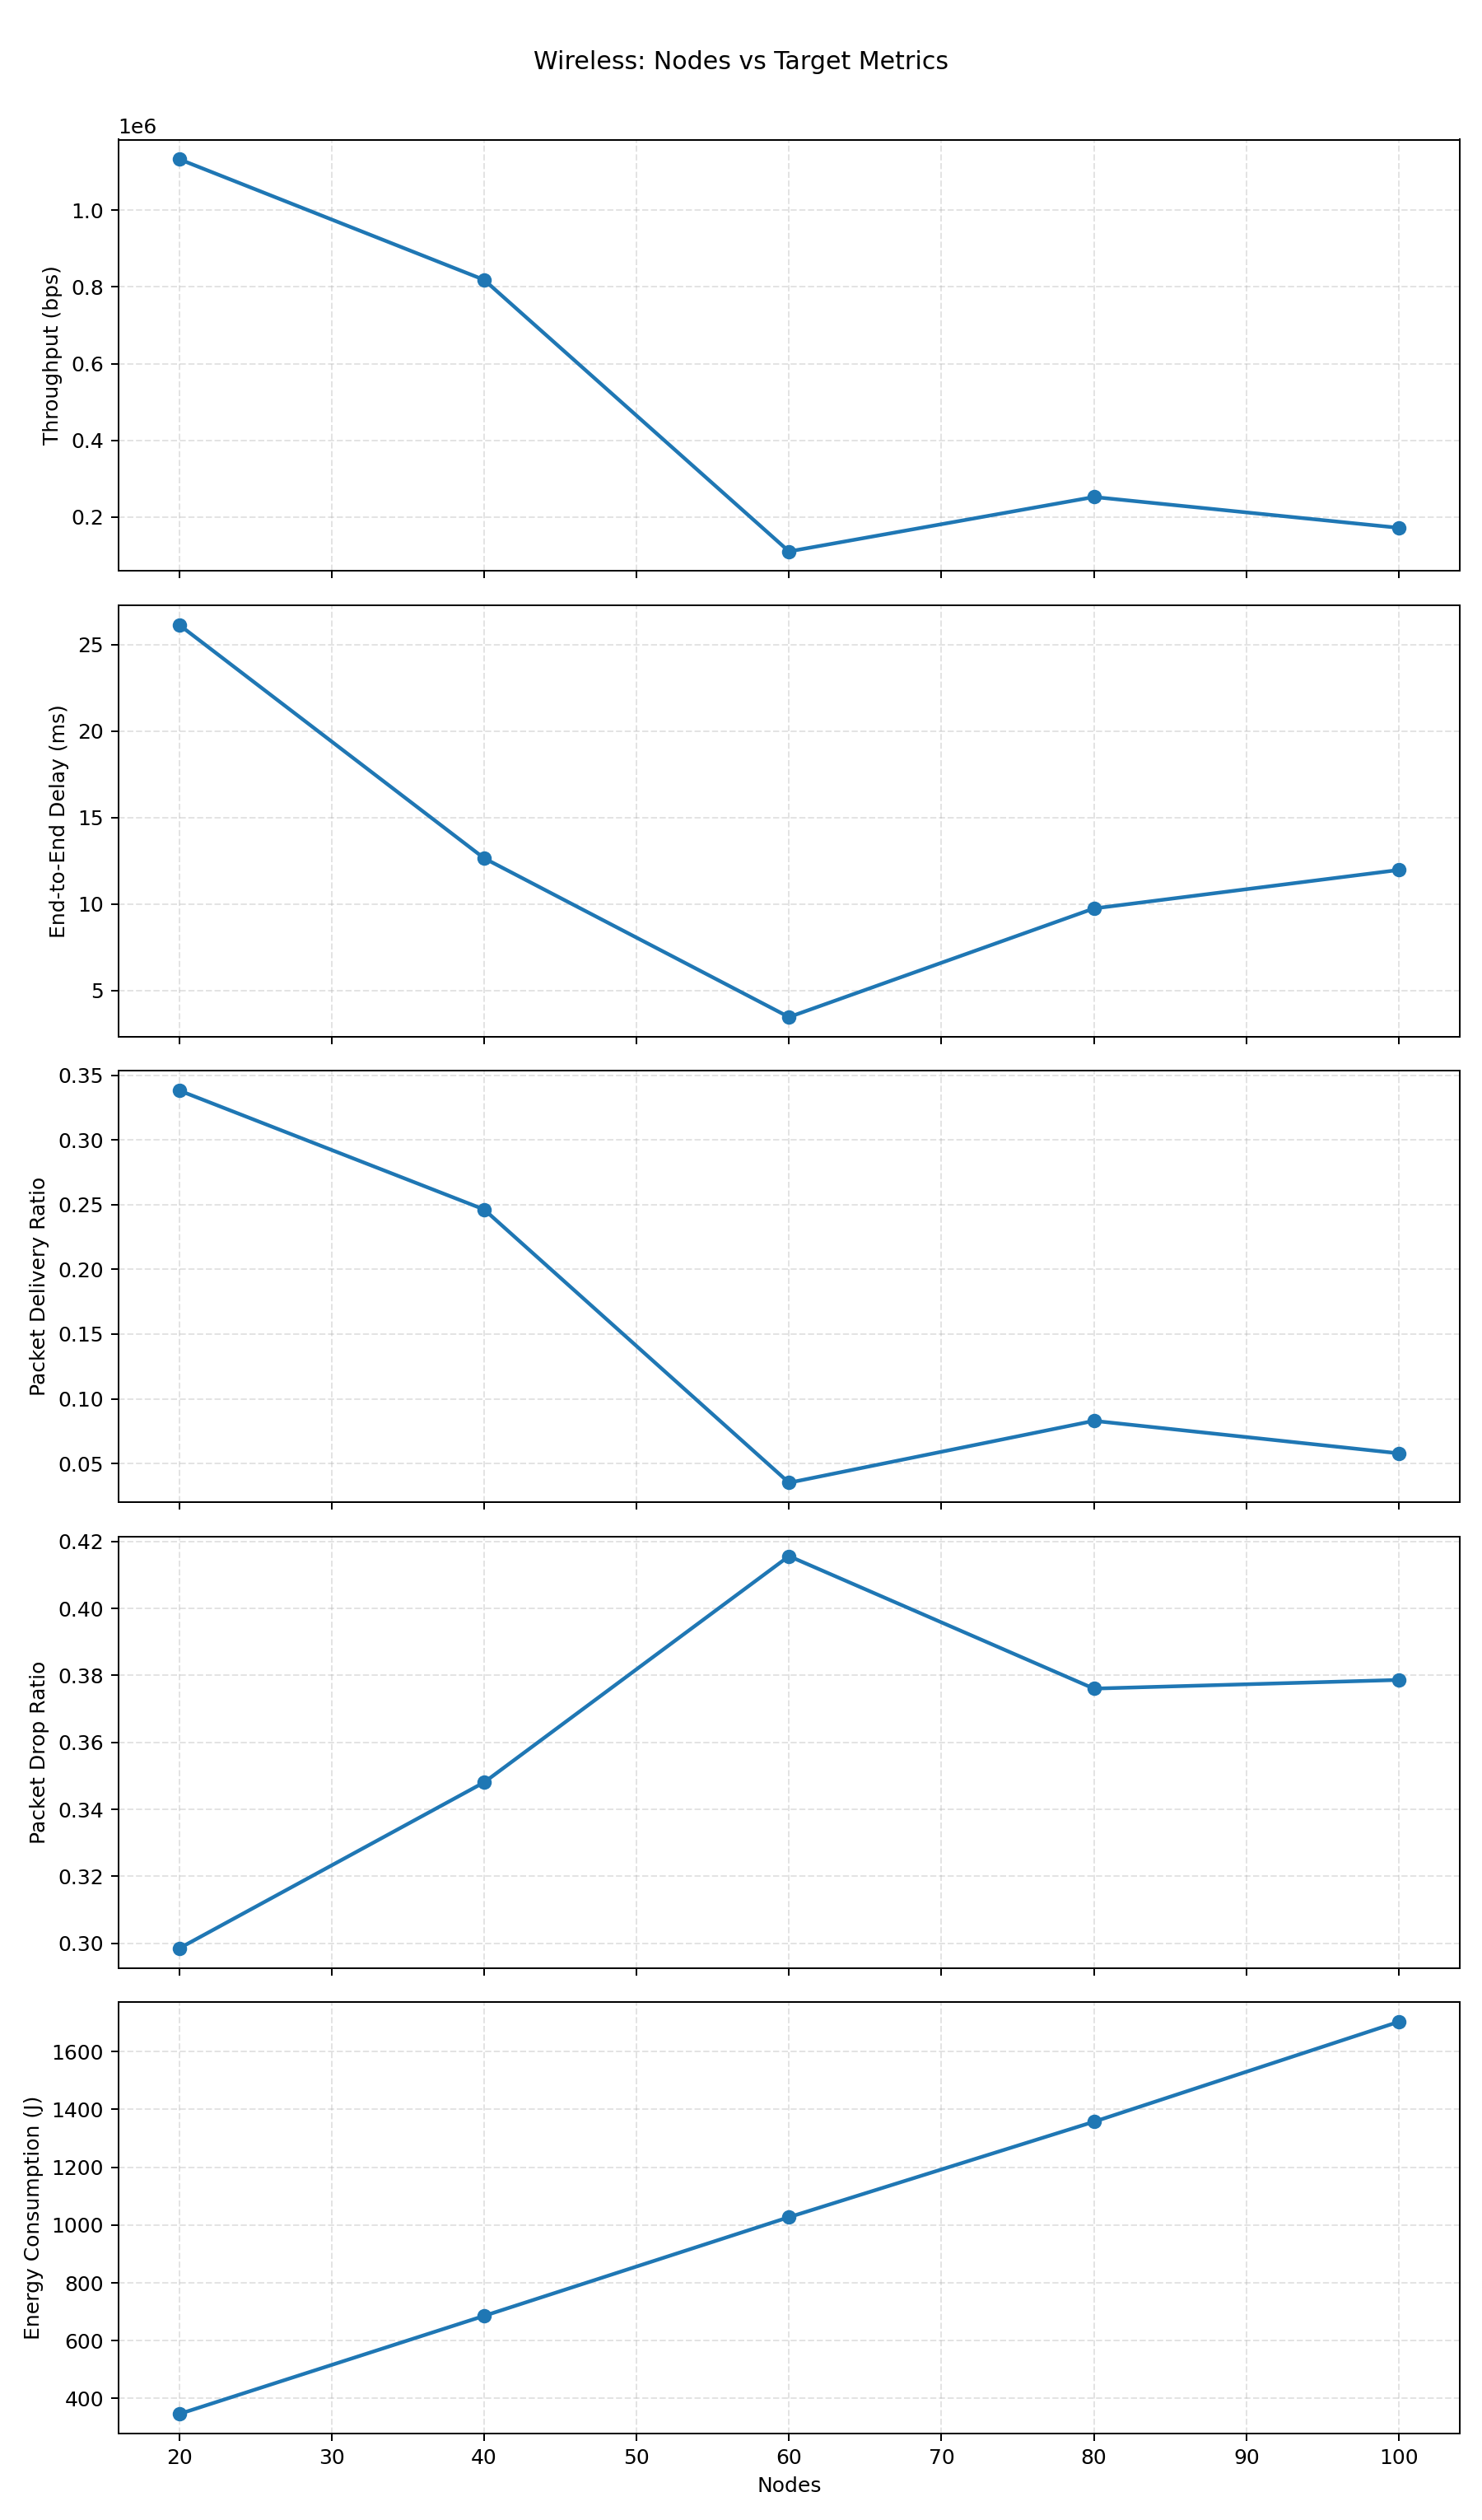
\includegraphics[height=0.9\textheight,keepaspectratio]{../results/wireless-csvs/plot-nodes-metrics.png}
    \caption{Wireless: Performance vs Number of Nodes}
\end{figure}

Increasing node density initially improves connectivity but eventually leads to congestion, reducing throughput and PDR while increasing delay and energy consumption.

\begin{table}[H]
    \centering
    \small
    \caption{Wireless node sweep results}
    \begin{tabular}{cccccc}
        \toprule
        Nodes & Throughput (bps) & Delay (ms) & PDR & Drop Ratio & Energy (J) \\
        \midrule
        20 & 513432 & 6.18 & 0.6896 & 0.0766 & 338.63 \\
        40 & 205848 & 17.92 & 0.2819 & 0.3014 & 679.70 \\
        60 & 176688 & 11.21 & 0.2424 & 0.3289 & 1010.64 \\
        80 & 81216 & 6.24 & 0.1157 & 0.3876 & 1342.05 \\
        100 & 77976 & 12.71 & 0.1133 & 0.3738 & 1680.03 \\
        \bottomrule
    \end{tabular}
\end{table}

\subsection{Wired Network Results}

\subsubsection{Effect of PPS}

\begin{figure}[H]
    \centering
    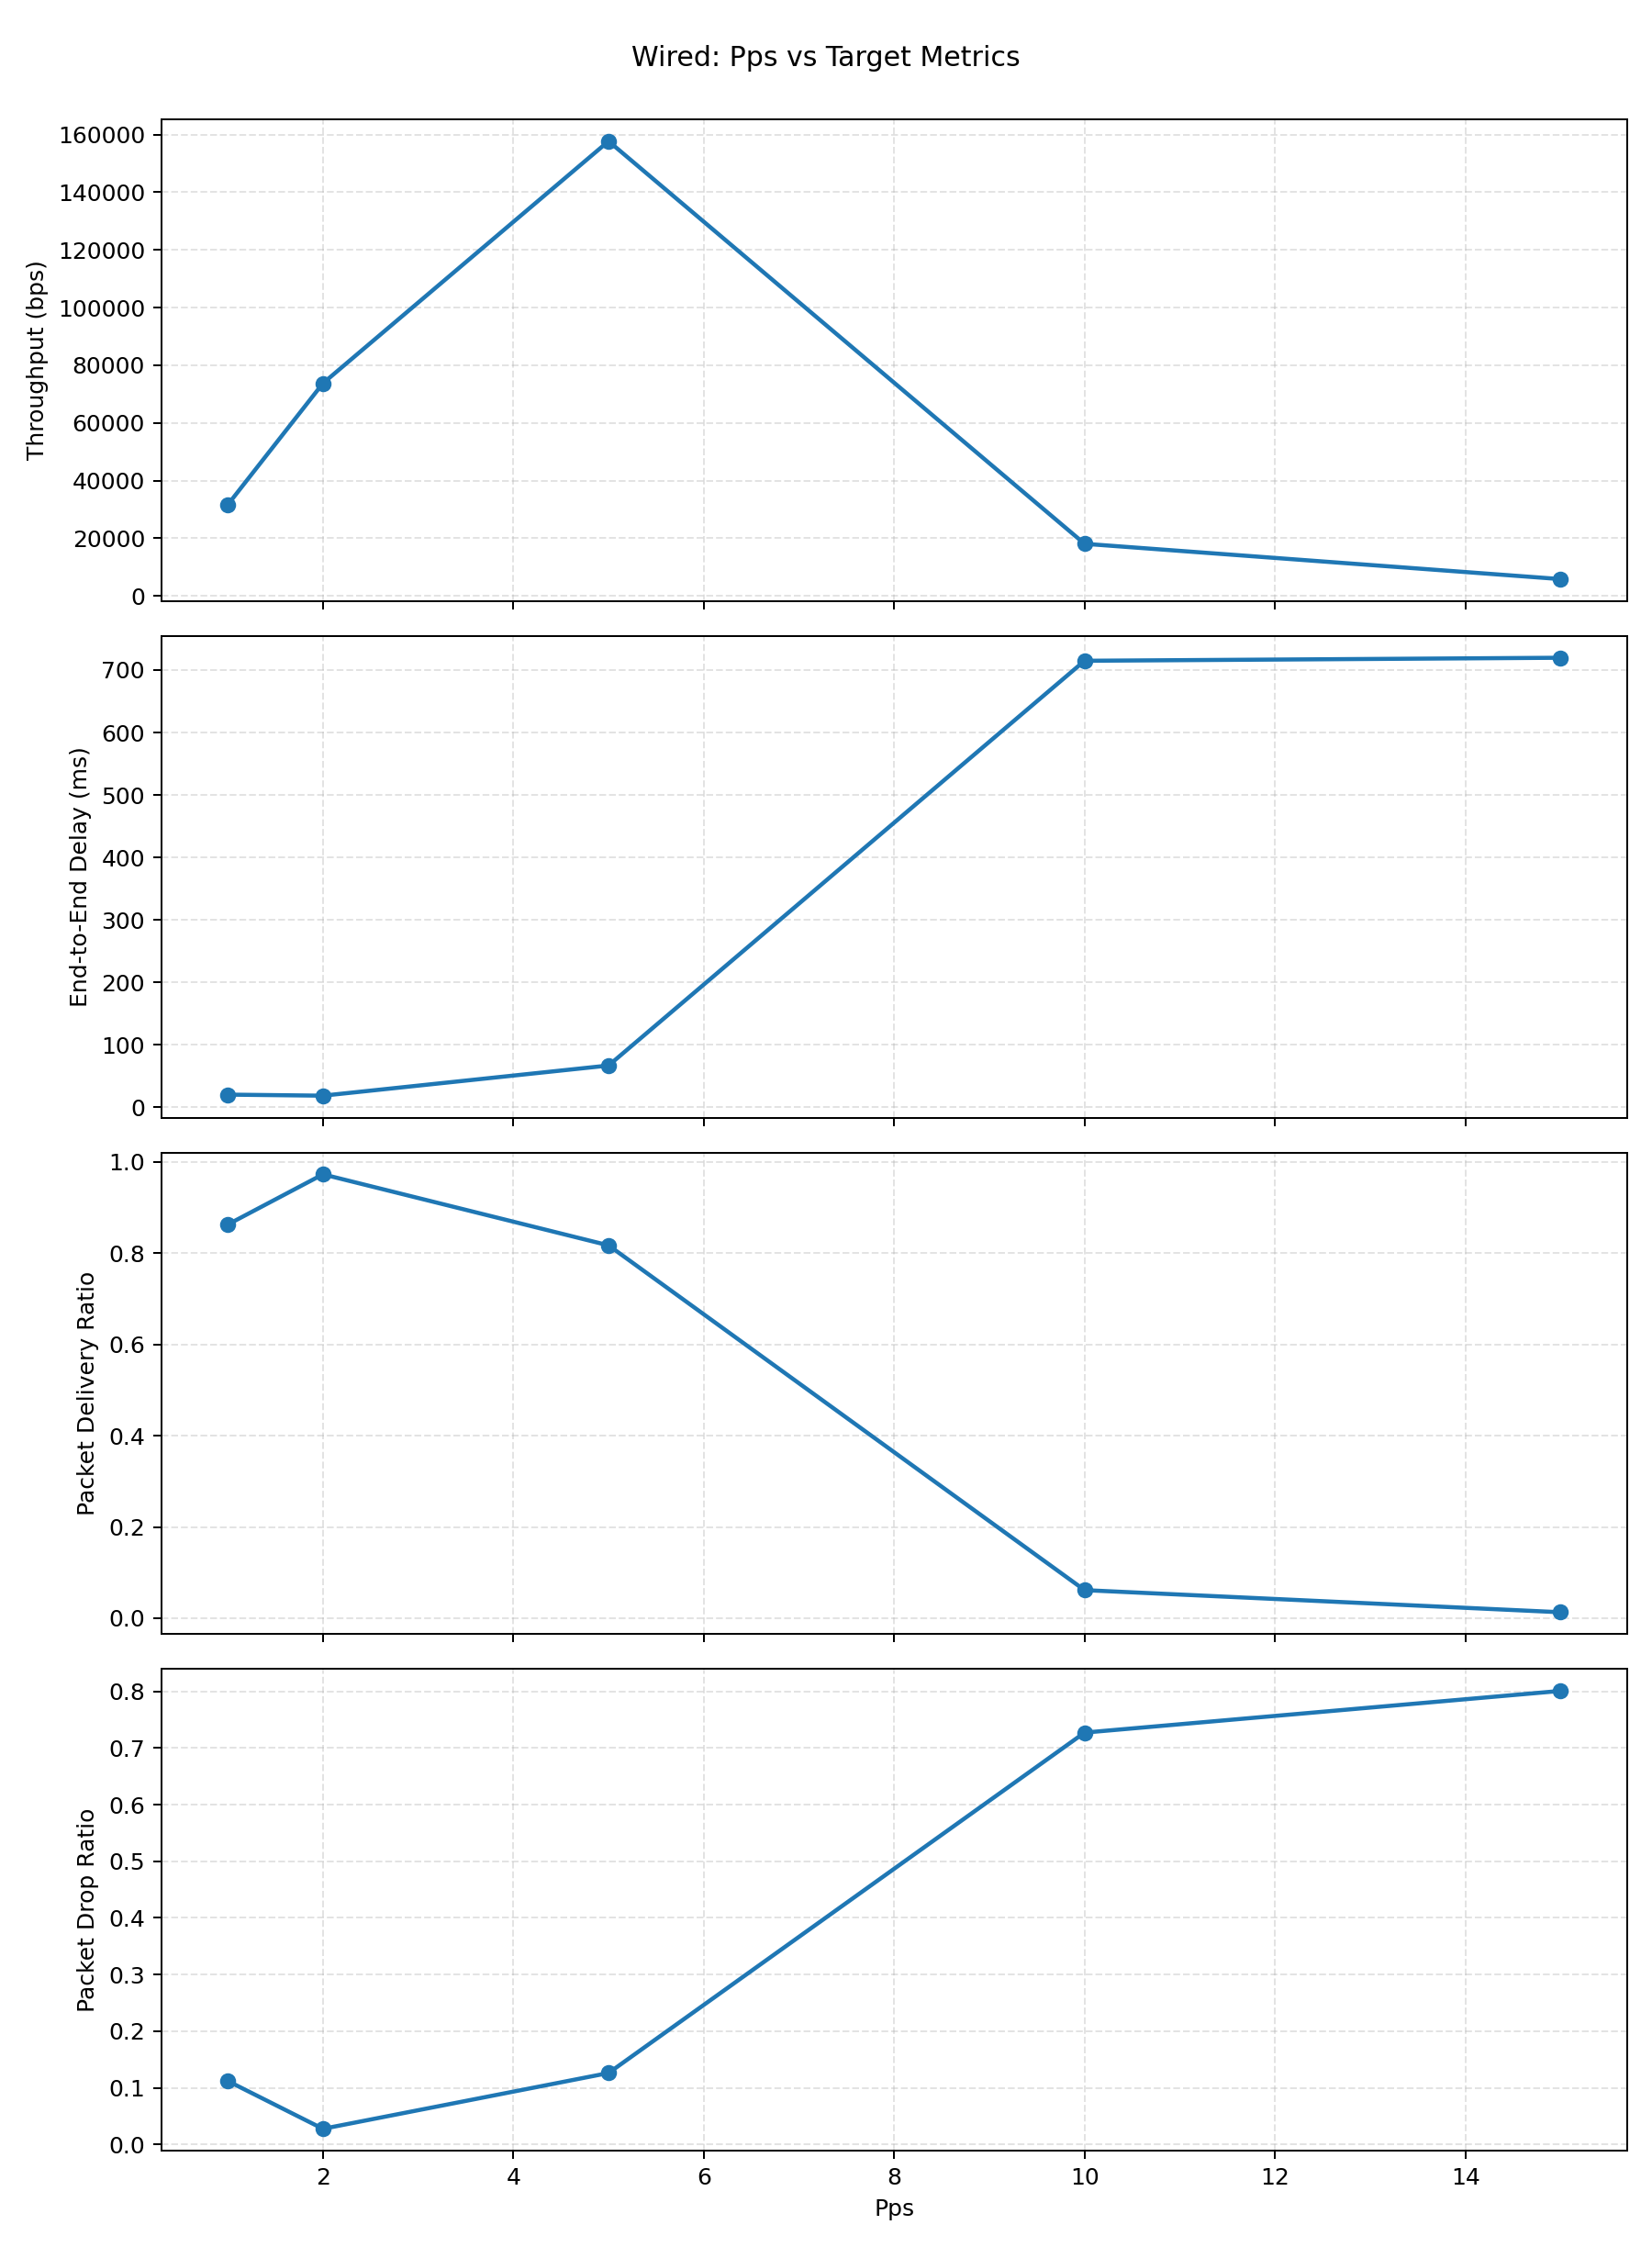
\includegraphics[height=0.9\textheight,keepaspectratio]{../results/wired-csvs/plot-pps-metrics.png}
    \caption{Wired: Performance vs PPS}
\end{figure}

Throughput increases up to a threshold and then drops sharply due to buffer overflow and congestion. Delay increases significantly at higher PPS values.

\begin{table}[H]
    \centering
    \small
    \caption{Wired PPS sweep results}
    \begin{tabular}{ccccc}
        \toprule
        PPS & Throughput (bps) & Delay (ms) & PDR & Drop Ratio \\
        \midrule
        100 & 109728 & 54.12 & 0.9525 & 0.0475 \\
        200 & 228600 & 12.39 & 0.9854 & 0.0146 \\
        300 & 233064 & 289.45 & 0.6855 & 0.2700 \\
        400 & 215496 & 353.41 & 0.4886 & 0.4445 \\
        500 & 205344 & 419.75 & 0.3670 & 0.5773 \\
        \bottomrule
    \end{tabular}
\end{table}

\subsubsection{Effect of Number of Flows}

\begin{figure}[H]
    \centering
    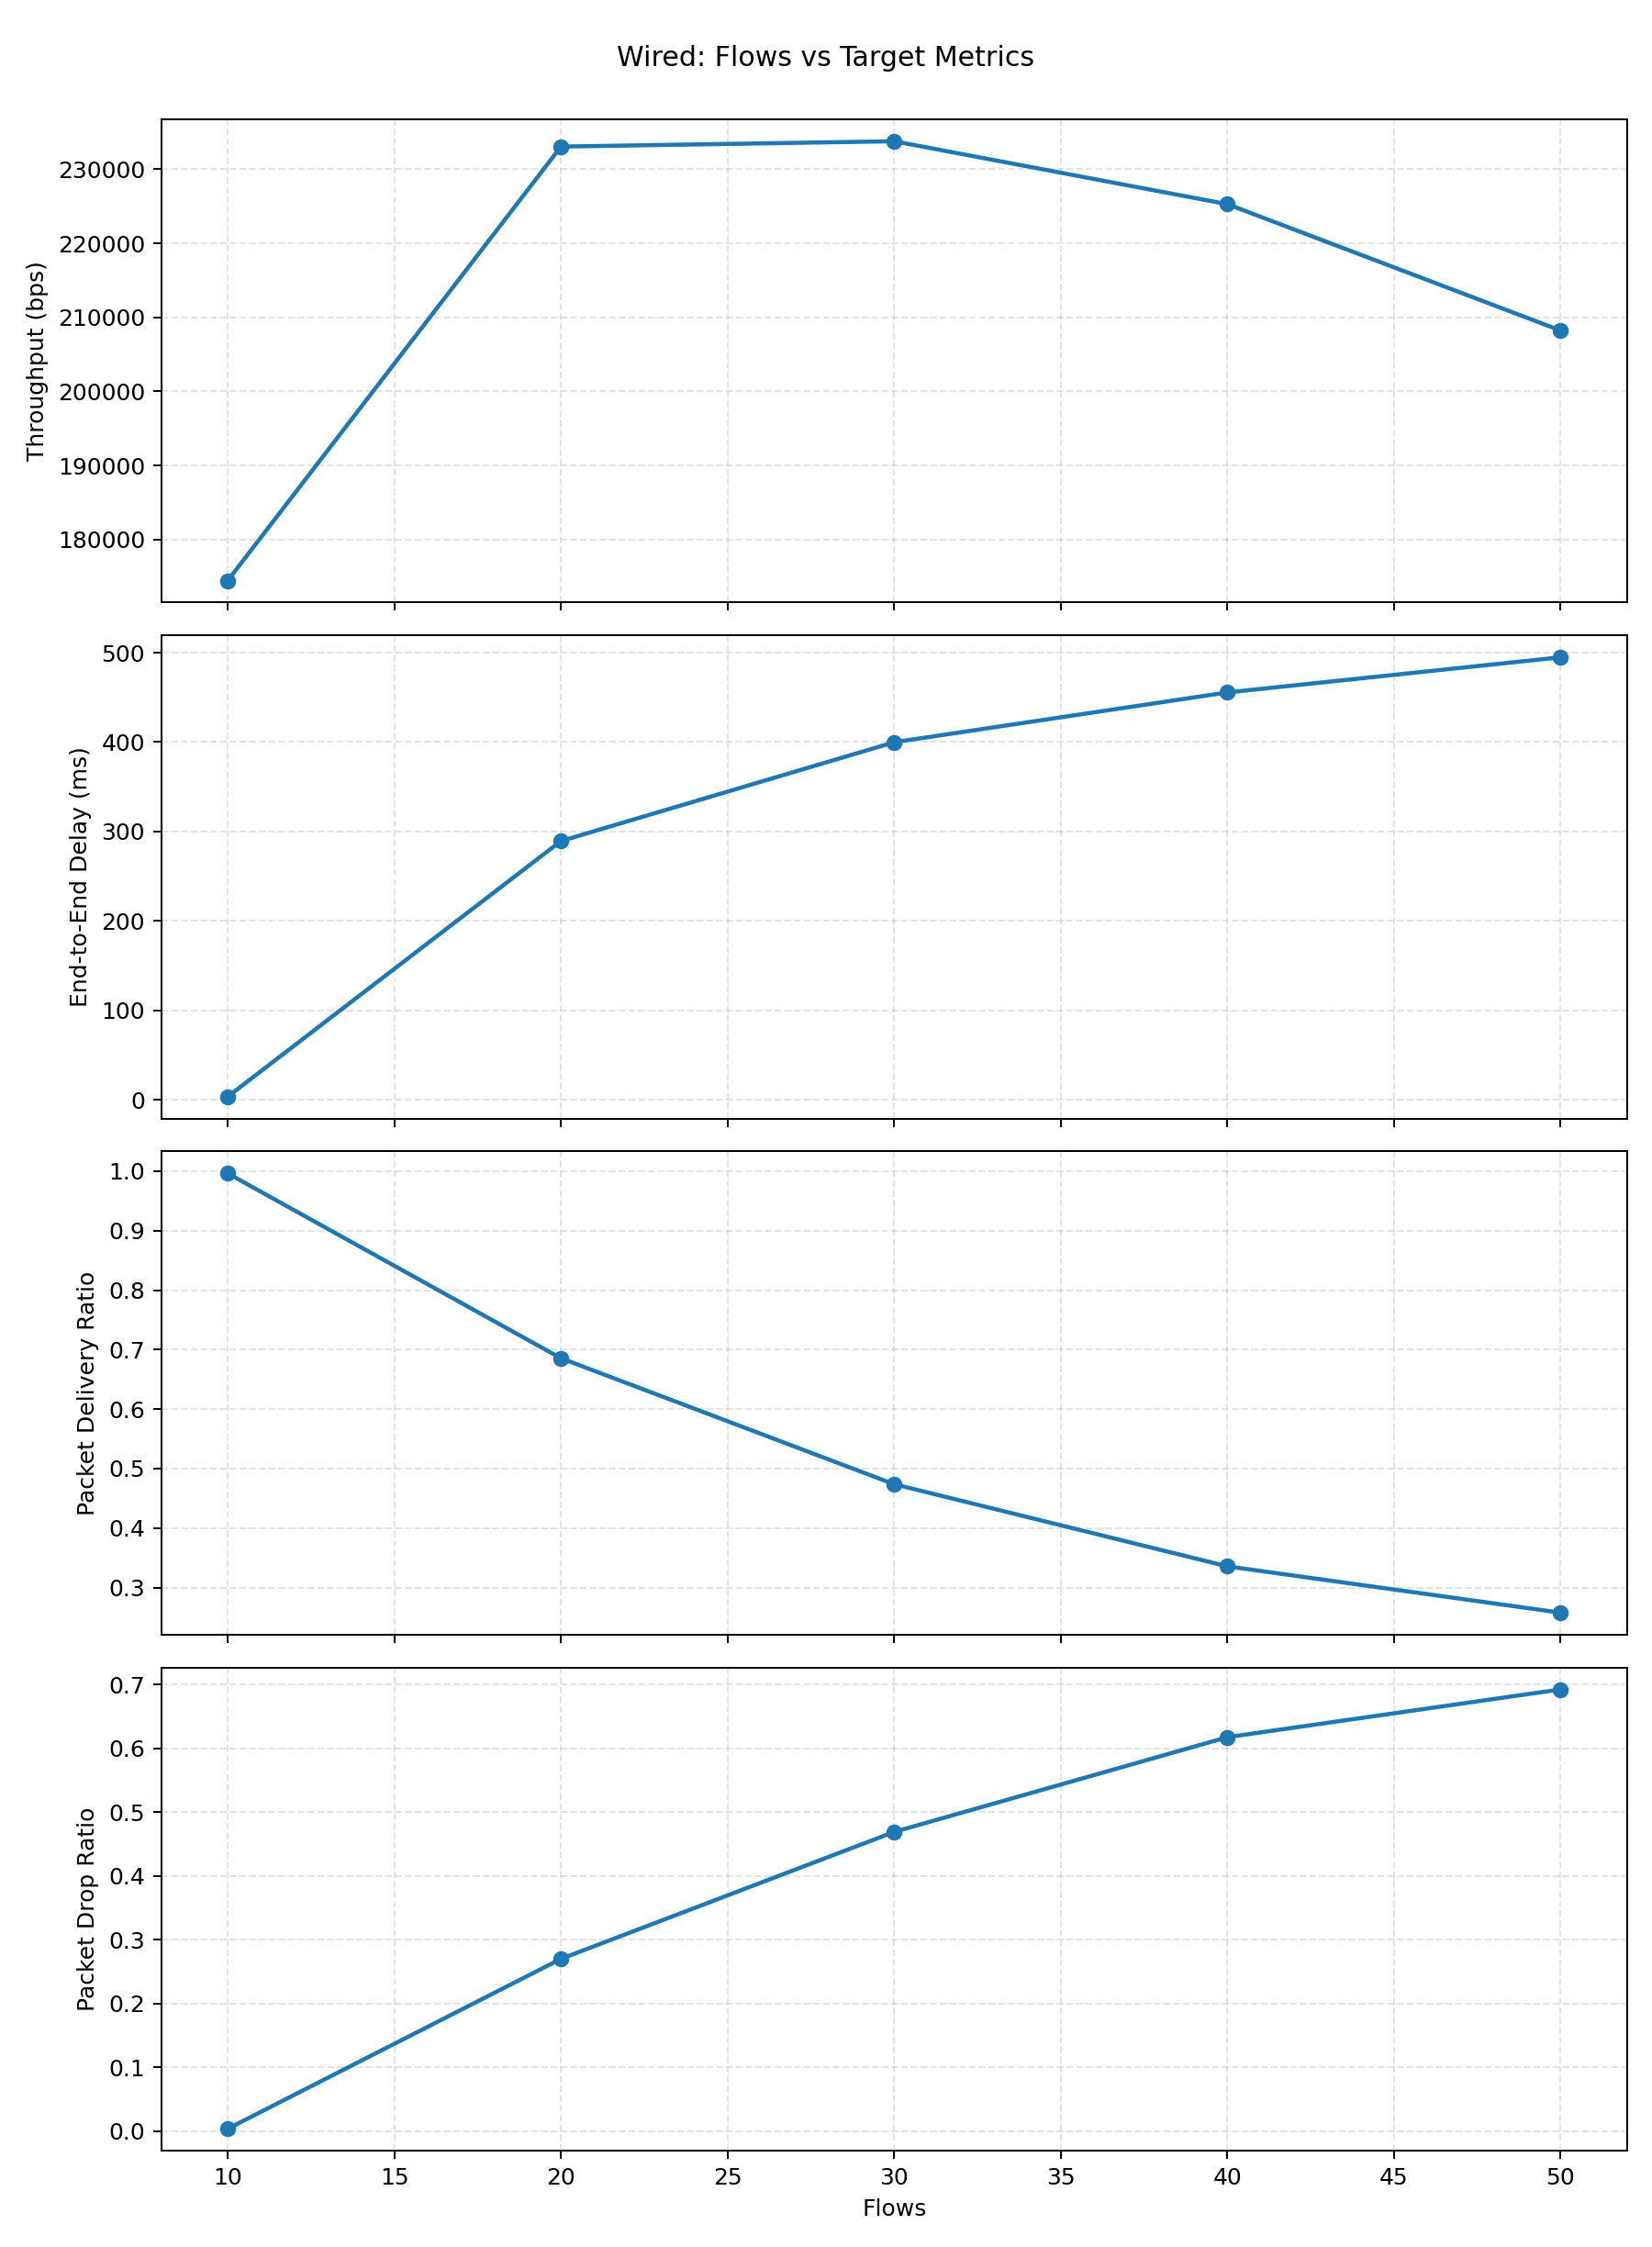
\includegraphics[height=0.9\textheight,keepaspectratio]{../results/wired-csvs/plot-flows-metrics.png}
    \caption{Wired: Performance vs Number of Flows}
\end{figure}

As flows increase, throughput decreases due to contention. Delay and packet drop ratio increase significantly.

\begin{table}[H]
    \centering
    \small
    \caption{Wired flow sweep results}
    \begin{tabular}{ccccc}
        \toprule
        Flows & Throughput (bps) & Delay (ms) & PDR & Drop Ratio \\
        \midrule
        10 & 174456 & 3.76 & 0.9963 & 0.0037 \\
        20 & 233064 & 289.45 & 0.6855 & 0.2700 \\
        30 & 233784 & 399.86 & 0.4737 & 0.4691 \\
        40 & 225288 & 455.52 & 0.3357 & 0.6176 \\
        50 & 208224 & 494.76 & 0.2578 & 0.6924 \\
        \bottomrule
    \end{tabular}
\end{table}

\subsubsection{Effect of Number of Nodes}

\begin{figure}[H]
    \centering
    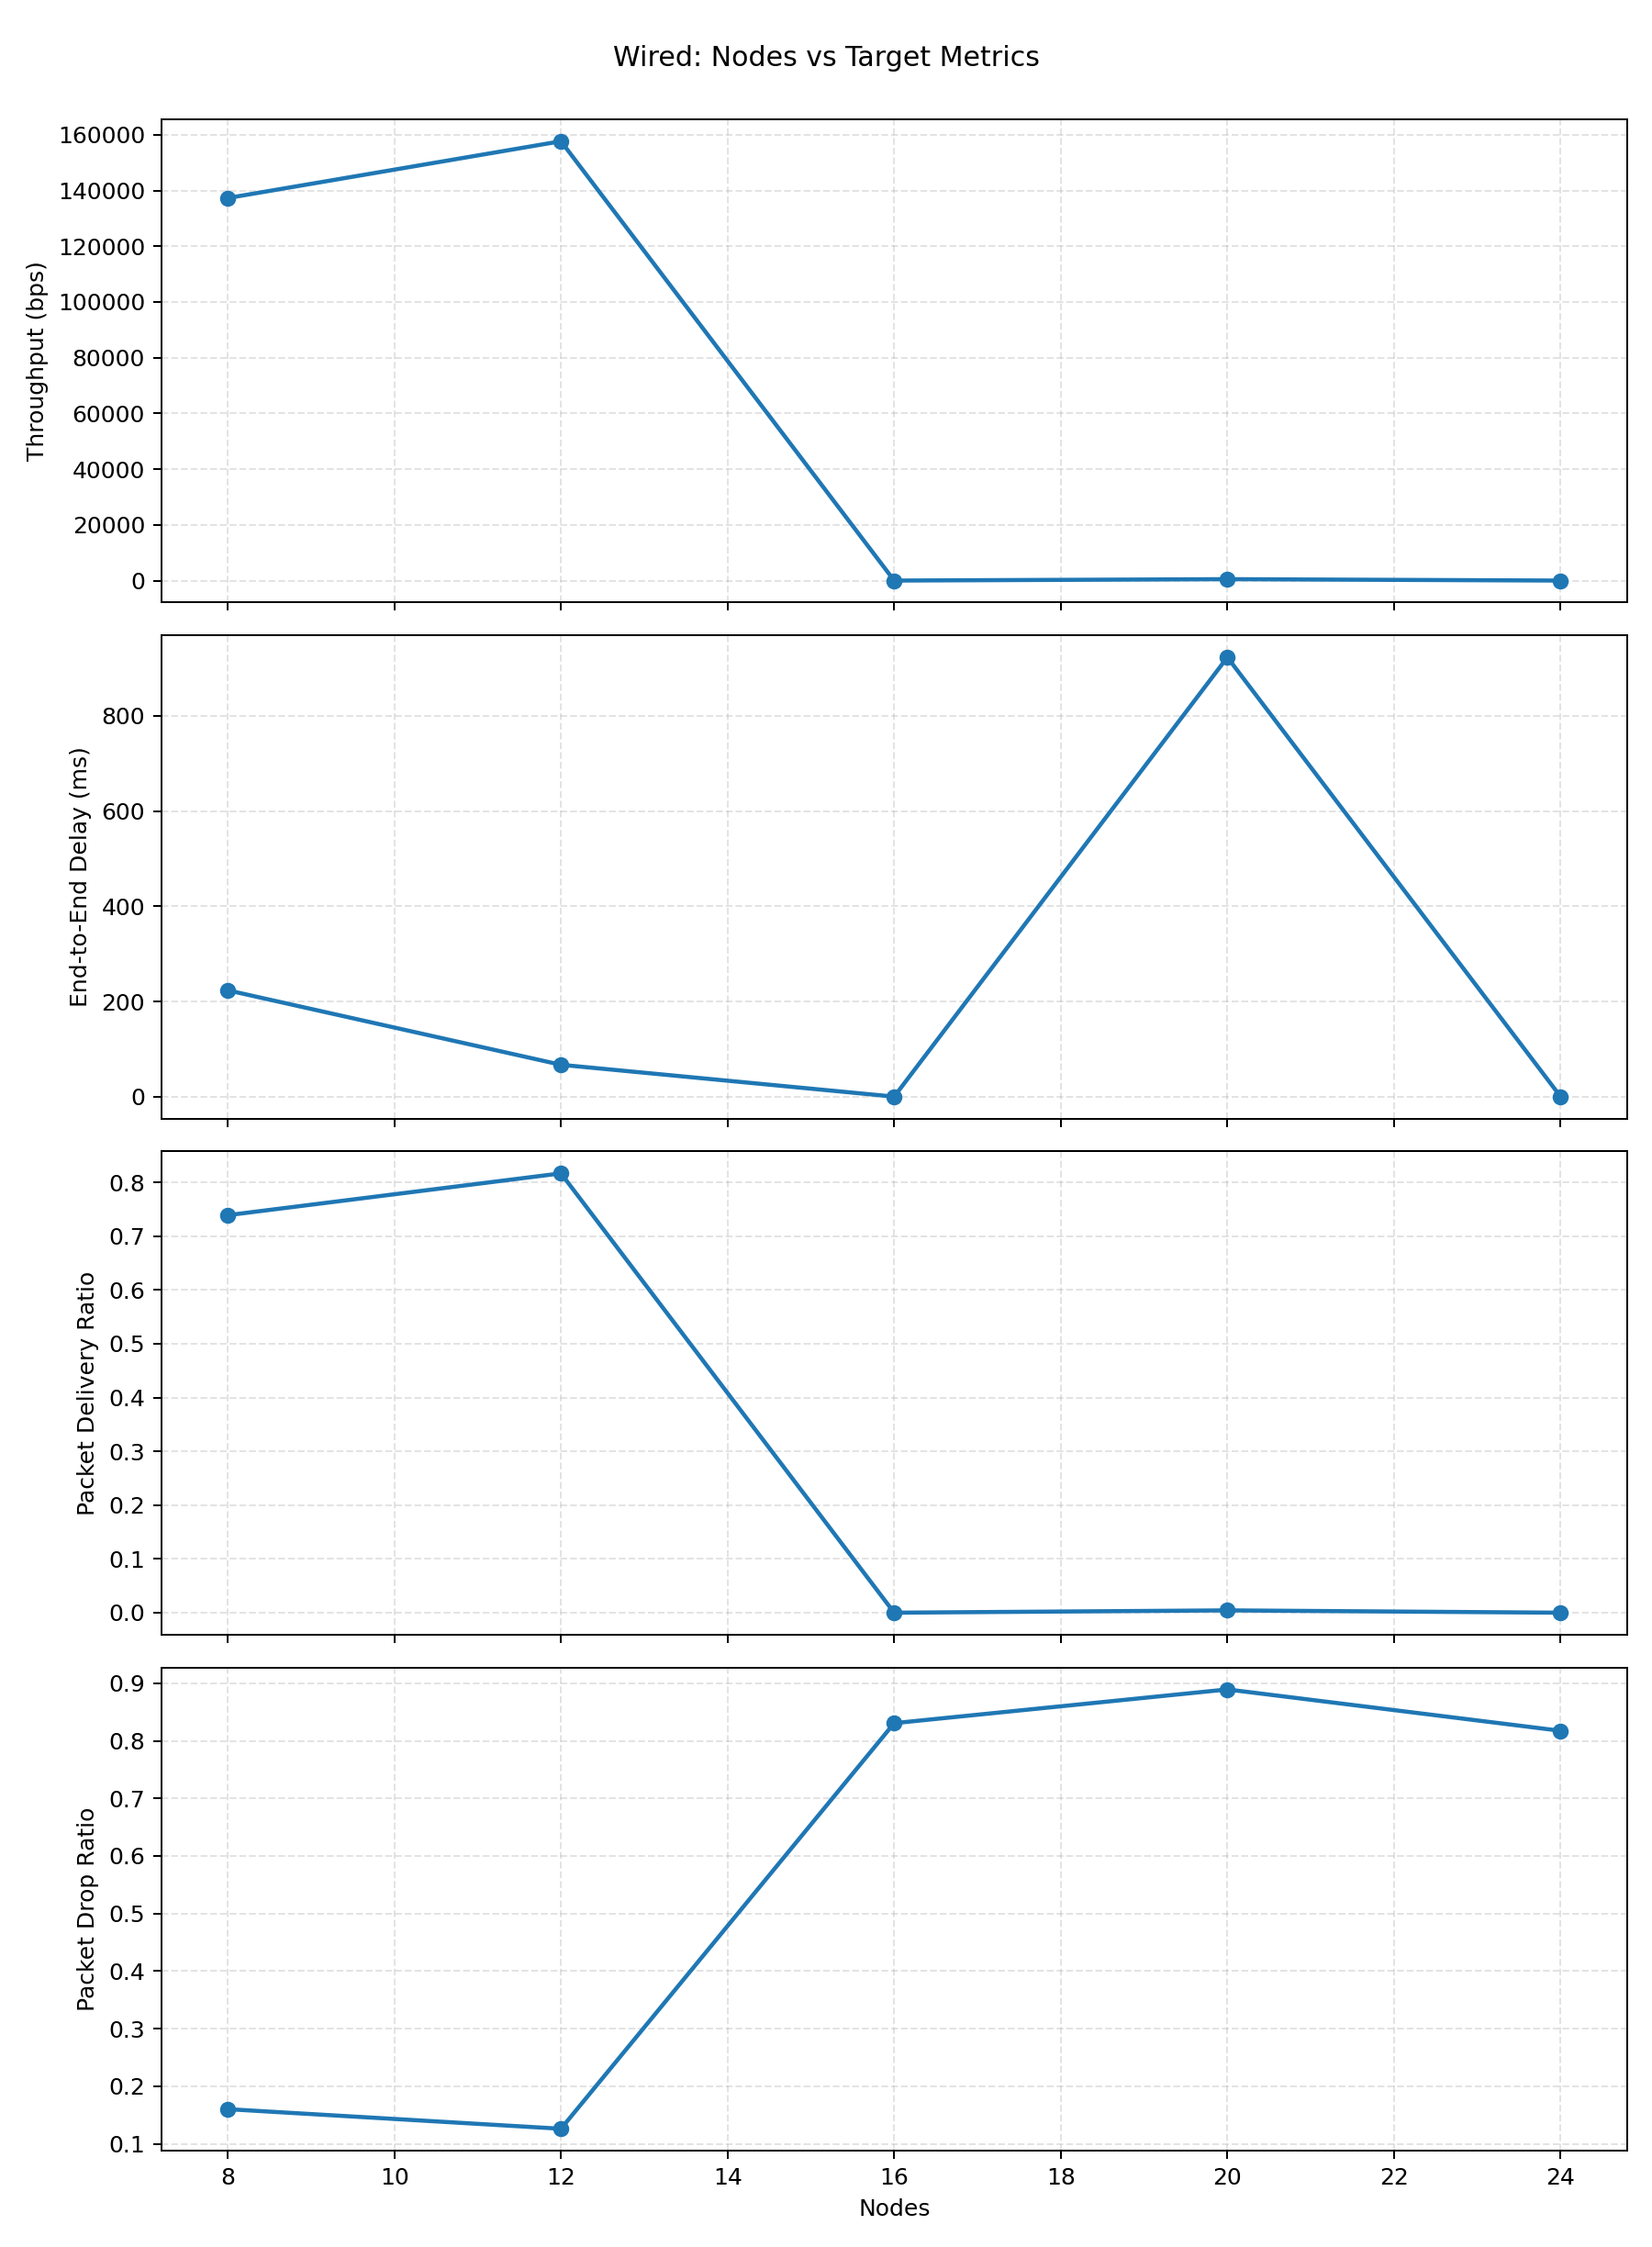
\includegraphics[height=0.9\textheight,keepaspectratio]{../results/wired-csvs/plot-nodes-metrics.png}
    \caption{Wired: Performance vs Number of Nodes}
\end{figure}

Higher node counts result in severe degradation in throughput and reliability due to routing overhead and congestion.

\begin{table}[H]
    \centering
    \small
    \caption{Wired node sweep results}
    \begin{tabular}{ccccc}
        \toprule
        Nodes & Throughput (bps) & Delay (ms) & PDR & Drop Ratio \\
        \midrule
        20 & 233064 & 289.45 & 0.6855 & 0.2700 \\
        40 & 48456 & 686.84 & 0.1417 & 0.7904 \\
        60 & 2592 & 940.10 & 0.0114 & 0.8980 \\
        80 & 1728 & 590.31 & 0.0109 & 0.9460 \\
        100 & 0 & 0.00 & 0.0000 & 0.7985 \\
        \bottomrule
    \end{tabular}
\end{table}

\section{Summary Findings}

\begin{itemize}
    \item AOMDV performs well under moderate load conditions.
    \item High PPS and flow counts lead to congestion and performance degradation.
    \item Mobility negatively impacts routing stability in wireless networks.
    \item Increasing nodes improves connectivity initially but degrades performance beyond a threshold.
    \item Wired networks show sharper performance drops under heavy load compared to wireless networks.
\end{itemize}

\section{Discussion and Reflection}

The results highlight the limitations of AOMDV under high traffic and dense network conditions. While multipath routing improves resilience, it introduces additional overhead that becomes significant under heavy load.

The deviation from the originally specified parameters was necessary due to:

\begin{itemize}
    \item Hardware limitations preventing large-scale simulations
    \item Excessive congestion causing unstable or non-converging simulations
\end{itemize}

This adjustment ensured meaningful and stable results.

From the observations:

\begin{itemize}
    \item There exists an optimal operating region for AOMDV
    \item Beyond this region, performance degrades rapidly
    \item Trade-offs between throughput, delay, and reliability are clearly visible
\end{itemize}

Future work could explore:

\begin{itemize}
    \item Comparison with other routing protocols (AODV, DSR)
    \item Optimization techniques for congestion control
    \item Adaptive routing based on network conditions
\end{itemize}

\section{Conclusion}

This study demonstrates that AOMDV is effective in moderate network conditions but struggles under high load and dense deployments. Careful parameter tuning is essential to achieve optimal performance in both wired and wireless environments.

\end{document}